\usepackage{fancyhdr}
%\usepackage{mu}
\usepackage{wasysym}
\usepackage{bitset}% Preambel mit Einstellungen importieren
% Document type and used packages
\documentclass[open=right, % Sorgt für Umbruch bei Chapter (any erzeugt keine Leerseiten) -> Kapitel darf nur auf der rechten Seite beginnen
    paper=A4,               % DIN-A4-Papier
    a4paper,                % DIN-A4-Papier
    12pt,                   % Schriftgöße
    headings=small,         % Kleine Überschriften
    headsepline=true,       % Trennlinie am Kopf der Seite
    footsepline=false,      % Keine Trennlinie am Fuß der Seite
    bibliography=totoc,     % Literaturverzeichnis in das Inhaltsverzeichnis aufnehmen
    twoside=off,            % Für doppelseitigen Druck auf on stellen, off für einseitig
    DIV=7,                  % Verhältnis der Ränder zum bedruckten Bereich
    chapterprefix=false,     % Kapitel x vor dem Kapitelnamen
    cleardoublepage=plain]{scrbook}

% Pakete einbinden, die benötigt werden
\usepackage{scrlayer-scrpage}
\usepackage[utf8]{inputenc}       % Dateien in UTF-8 benutzen
\usepackage[T1]{fontenc}          % Zeichenkodierung
\usepackage{graphicx}             % Bilder einbinden
\usepackage[main=ngerman, english]{babel}       % Deutsch und Englisch unterstützen
\usepackage{xcolor}               % Color support
\usepackage{amsmath}              % Matheamtische Formeln
\usepackage{amsfonts}             % Mathematische Zeichensätze
\usepackage{amssymb}              % Mathematische Symbole
\usepackage{float}                % Fließende Objekte (Tabellen, Grafiken etc.)
\usepackage{booktabs}             % Korrekter Tabellensatz
\usepackage[printonlyused, withpage, footnote]{acronym}  % Abkürzungsverzeichnis [nur verwendete Abkürzugen]
\usepackage{makeidx}              % Sachregister
\usepackage{listings}             % Source Code listings
\usepackage{listingsutf8}         % Listings in UTF8
\usepackage[hang,font={sf,footnotesize},labelfont={footnotesize,bf}]{caption} % Beschriftungen
\usepackage[scaled]{helvet}       % Schrift Helvetia laden
\usepackage[absolute]{textpos}	  % Absolute Textpositionen (für Deckblatt)
\usepackage{calc}                 % Berechnung von Positionen
\usepackage{blindtext}            % Blindtexte
\usepackage[bottom=40mm,left=35mm,right=35mm,top=30mm]{geometry} % Ränder ändern
\usepackage{setspace}             % Abstände korrigieren
\usepackage{ifthen}               % Logische Bedingungen mit ifthenelse
\usepackage{scrhack}              % Get rid of tocbasic warnings
\usepackage[pagebackref=false,german]{hyperref}  % Hyperlinks
\usepackage[all]{hypcap}          % Korrekte Verlinkung von Floats
\usepackage[autostyle=true,german=quotes]{csquotes}   % Zitate
\usepackage[backend=biber,
  isbn=true,                     % ISBN nicht anzeigen, gleiches geht mit nahezu allen anderen Feldern
  sortlocale=de_DE,               % Sortierung der Einträge für Deutsch
  %sortlocale=en_US,              % Sortierung der Einträge für Englisch
  autocite=inline,                % regelt Aussehen für \autocite (inline=\parancite)
  hyperref=true,                  % Hyperlinks für Ziate
  style=ieee                     % Zitate als Zahlen [1]
  %style=alphabetic               % Zitate als Kürzel und Jahr [Ein05]
  %style=authoryear                % Zitate Author und Jahr [Einstein (1905)]
  %style=LNI
]{biblatex}                       % Literaturverwaltung mit BibLaTeX
\usepackage{rotating}             % Seiten drehen
\usepackage{harveyballs}          % Harveyballs
\usepackage{tcolorbox}
\usepackage[export]{adjustbox}
\usepackage{subcaption}
\usepackage{color}
\usepackage{colortbl}
\usepackage{wrapfig}
\usepackage{todonotes}
\usepackage{tabularx}
\newcolumntype{b}{>{\hsize=1.2\hsize}X}
\newcolumntype{m}{>{\hsize=.5\hsize}X}
\newcolumntype{s}{>{\hsize=.3\hsize}X}
\usepackage{tikz}


\setlength{\bibitemsep}{1em}     % Abstand zwischen den Literaturangaben
\setlength{\bibhang}{2em}        % Einzug nach jeweils erster Zeile

% Trennung von URLs im Literaturverzeichnis (große Werte [> 10000] verhindern die Trennung)
\defcounter{biburlnumpenalty}{10} % Strafe für Trennung in URL nach Zahl
\defcounter{biburlucpenalty}{500}  % Strafe für Trennung in URL nach Großbuchstaben
\defcounter{biburllcpenalty}{500}  % Strafe für Trennung in URL nach Kleinbuchstaben

% Farben definieren
\definecolor{linkblue}{RGB}{0, 0, 100}
\definecolor{linkblack}{RGB}{0, 0, 0}
\definecolor{comment}{RGB}{63, 127, 95}
\definecolor{darkgreen}{RGB}{14, 144, 102}
\definecolor{darkblue}{RGB}{0,0,168}
\definecolor{darkred}{RGB}{128,0,0}
\definecolor{javadoccomment}{RGB}{0,0,240}
\definecolor{Gray}{RGB}{242,242,242}

% Einstellungen für das Hyperlink-Paket
\hypersetup{
    colorlinks=true,      % Farbige links verwenden
%    allcolors=linkblue,
    linktoc=all,          % Links im Inhaltsverzeichnis
    linkcolor=linkblack,  % Querverweise
    citecolor=linkblack,  % Literaturangaben
	filecolor=linkblack,  % Dateilinks
	urlcolor=linkblack    % URLs
}

% Einstellungen für Quelltexte
\definecolor{backcolour}{rgb}{0.95,0.95,0.92}
\definecolor{codegray}{rgb}{0.5,0.5,0.5}
\lstset{
      xleftmargin=0.1cm,
      basicstyle=\footnotesize\ttfamily,
      keywordstyle=\color{darkgreen},
      identifierstyle=\color{darkblue},
      commentstyle=\color{comment},
      stringstyle=\color{darkred},
      tabsize=2,
      lineskip={2pt},
      columns=flexible,
      inputencoding=utf8,
      captionpos=b,
      backgroundcolor=\color{backcolour},   
      breakautoindent=true,
	  breakindent=2em,
	  breaklines=true,
	  prebreak=,
	  postbreak=,
      numbers=left,                    
      numbersep=5pt,  
      numberstyle=\tiny\color{codegray},  
      showspaces=false,      % Keine Leerzeichensymbole
      showtabs=false,        % Keine Tabsymbole
      showstringspaces=false,% Leerzeichen in Strings
      morecomment=[s][\color{javadoccomment}]{/**}{*/},
      literate={Ö}{{\"O}}1 {Ä}{{\"A}}1 {Ü}{{\"U}}1 {ß}{{\ss}}2 {ü}{{\"u}}1 {ä}{{\"a}}1 {ö}{{\"o}}1
}


\urlstyle{same}

% Einstellungen für Überschriften
\renewcommand*{\chapterformat}{%
  \Large~\thechapter. ~   		% Große Schrift
  \vspace{0.3cm}               	% Abstand zum Titel des Kapitels
}

% Abstände für die Überschriften setzen
\renewcommand{\chapterheadstartvskip}{\vspace*{2.6cm}}
\renewcommand{\chapterheadendvskip}{\vspace*{1.5cm}}

\RedeclareSectionCommand[
  beforeskip=-1.8\baselineskip,
  afterskip=0.25\baselineskip]{section}

\RedeclareSectionCommand[
  beforeskip=-1.8\baselineskip,
  afterskip=0.15\baselineskip]{subsection}

\RedeclareSectionCommand[
  beforeskip=-1.8\baselineskip,
  afterskip=0.15\baselineskip]{subsubsection}


% In der Kopfzeile nur die kurze Kapitelbezeichnung (ohne Kapitel davor)
\renewcommand*\chaptermarkformat{\thechapter\autodot\enskip}
\automark[chapter]{chapter}

% Einstellungen für Schriftarten
\setkomafont{pagehead}{\normalfont\sffamily}
\setkomafont{pagenumber}{\normalfont\sffamily}
\setkomafont{paragraph}{\sffamily\bfseries\small}
\setkomafont{subsubsection}{\sffamily\itshape\bfseries\small}
\addtokomafont{footnote}{\footnotesize}
\setkomafont{chapter}{\LARGE\selectfont\bfseries}

% Wichtige Abstände
\setlength{\parskip}{0.2cm}  % 2mm Abstand zwischen zwei Absätzen
\setlength{\parindent}{0mm}  % Absätze nicht einziehen
\clubpenalty = 10000         % Keine "Schusterjungen"
\widowpenalty = 10000        % Keine "Hurenkinder"
\displaywidowpenalty = 10000 % Keine "Hurenkinder"
\renewcommand{\footnotesize}{\fontsize{9}{10}\selectfont} % Größe der Fußnoten
\setlength{\footnotesep}{8pt} % Abstand zwischen den Fußnoten

% Index erzeugen
\makeindex

% Einfacher Font-Wechsel über dieses Makro
\newcommand{\changefont}[3]{
\fontfamily{#1} \fontseries{#2} \fontshape{#3} \selectfont}

% Eigenes Makro für Bilder
\newcommand{\bild}[3]{
\begin{figure}[h]
  \centering
  \includegraphics[width=#2]{#1}
  \caption{#3}
  \label{#1}
\end{figure}}

% Wo liegt Sourcecode?
\newcommand{\srcloc}{src/}

% Wo sind die Bilder?
\graphicspath{{bilder/}}

% Makros für typographisch korrekte Abkürzungen
\newcommand{\zb}[0]{z.\,B.\ }
\newcommand{\dahe}[0]{d.\,h.\ }
\newcommand{\ua}[0]{u.\,a.\ }

% Flags für Veröffentlichung und Sperrvermerk
\newboolean{hsmapublizieren}
\newboolean{hsmasperrvermerk}


% Dokumenteninfos importieren
% In docinfo.tex sind Titel, Autor, Abstract zu definieren
% -------------------------------------------------------
% Daten für die Arbeit
% Wenn hier alles korrekt eingetragen wurde, wird das Titelblatt
% automatisch generiert. D.h. die Datei titelblatt.tex muss nicht mehr
% angepasst werden.

\newcommand{\hsmasprache}{de} % de oder en für Deutsch oder Englisch
% Für korrekt sortierte Literatureinträge, noch preambel.tex anpassen
% und zwar bei \usepackage[main=ngerman, english]{babel},
% \usepackage[pagebackref=false,german]{hyperref}
% und \usepackage[autostyle=true,german=quotes]{csquotes}

% Titel der Arbeit auf Deutsch
\newcommand{\hsmatitelde}{Embedded Frontend-Entwicklung mit .Net Core und Blazor}

% Titel der Arbeit auf Englisch
\newcommand{\hsmatitelen}{Embedded Frontend-Development with .Net Core and Blazor}

% Weitere Informationen zur Arbeit
\newcommand{\hsmaort}{Offenburg}    % Ort
\newcommand{\hsmaautorvname}{William} % Vorname(n)
\newcommand{\hsmaautornname}{Mendat} % Nachname(n)
\newcommand{\hsmadatum}{28.02.2022} % Datum der Abgabe
\newcommand{\hsmajahr}{2022} % Jahr der Abgabe
\newcommand{\hsmafirma}{Junker Technologies} % Firma bei der die Arbeit durchgeführt wurde
\newcommand{\hsmabetreuer}{Prof. Dr.-Ing. Daniel Fischer, Hochschule Offenburg} % Betreuer an der
\newcommand{\hsmazweitkorrektor}{M. Sc. Adrian Junker, Junker Technologies} % Betreuer im
\newcommand{\hsmafakultaet}{EMI} % Fakultät
\newcommand{\hsmastudiengang}{AI} % Studiengangsabkürzung.
% Diese wird in titelblatt.tex definiert. Bisher AI, EI, MK und INFM. Bitte ergänzen.

% Zustimmung zur Veröffentlichung
\setboolean{hsmapublizieren}{true}   % Einer Veröffentlichung wird zugestimmt
\setboolean{hsmasperrvermerk}{false} % Die Arbeit hat keinen Sperrvermerk

% -------------------------------------------------------
% Abstract

% Kurze (maximal halbseitige) Beschreibung, worum es in der Arbeit geht auf Deutsch
\newcommand{\hsmaabstractde}{In dieser Abschlussarbeit wird eine Net Core Blazer Anwendung implementiert, um
somit einen Ersatz für die derzeit GUI-Entwicklung auf dem Raspberry Pi mit Qt
zu kreieren. Dabei werden verschiedene Ansätze implementiert, sowohl auf dem
Raspberry Pi als auch auf einem externen Server, um einen aussagekräftigen
Vergleich zwischen den hier verschiedenen Technologien zu schaffen. Ein großer
Teil dieser Ausarbeitung besteht darin, eine Laufzeitanalyse zu erstellen.

Die Arbeit gibt zunächst einen Einblick in den momentanen Stand der Technik, wie
bislang mit einem Raspberry Pi gearbeitet wurde, um dann zu veranschaulichen, wie
dass gleiche Verhalten mit Net Core und Blazer widergespiegelt werden kann.
Am Ende dieser Arbeit wird ein aussagekräftiges Fazit darüber abgegeben, ob die
Technologie Blazor für die Frontendentwicklung im Embedded Bereich zu gebrauchen ist.}

% Kurze (maximal halbseitige) Beschreibung, worum es in der Arbeit geht auf Englisch

\newcommand{\hsmaabstracten}{Englische Version von Lorem ipsum dolor sit amet, consetetur sadipscing elitr, sed diam nonumy eirmod tempor invidunt ut labore et dolore magna aliquyam erat, sed diam voluptua. At vero eos et accusam et justo duo dolores et ea rebum. Stet clita kasd gubergren, no sea takimata sanctus est Lorem ipsum dolor sit amet. Lorem ipsum dolor sit amet, consetetur sadipscing elitr, sed diam nonumy eirmod tempor invidunt ut labore et dolore magna aliquyam erat, sed diam voluptua. At vero eos et accusam et justo duo dolores et ea rebum. Stet clita kasd gubergren, no sea takimata sanctus est Lorem ipsum dolor sit amet.}


% Literatur-Datenbank
\addbibresource{literatur.bib}   % BibLaTeX-Datei mit Literaturquellen einbinden

\begin{document}
\frontmatter

% Römische Ziffern für die "Front-Matter"
\setcounter{page}{0}
\changefont{ptm}{m}{n}  % Times New Roman für den Fließtext
\renewcommand{\rmdefault}{ptm}

% Titelblatt
% -------------------------------------------------------
% In dieser Datei sollten eigentlich keine Veränderungen mehr
% notwendig sein.
% -------------------------------------------------------

\thispagestyle{empty}

% Fakultät
% -------------------------------------------------------
\ifthenelse{\equal{\hsmafakultaet}{EI}}%
  {\newcommand{\hsmafakultaetlangde}{Fakultät Elektrotechnik und Informationstechnik}%
   \newcommand{\hsmafakultaetlangen}{Department of Electrical Engineering and Computer Science}}{}
\ifthenelse{\equal{\hsmafakultaet}{EMI}}%
{\newcommand{\hsmafakultaetlangde}{Fakultät Elektrotechnik, Medizintechnik und Informatik}%
	\newcommand{\hsmafakultaetlangen}{Department of Electrical Engineering, Medical Engineering and Computer Science}}{}



\ifthenelse{\equal{\hsmastudiengang}{AI}}%
{\newcommand{\hsmastudienganglangde}{Angewandte Informatik}%
	\newcommand{\hsmastudienganglangen}{Applied Computer Science}%
	\newcommand{\hsmatypde}{BACHELORARBEIT}%
	\newcommand{\hsmatypen}{BACHELOR THESIS}%
	\newcommand{\hsmagrad}{\hsmabachelor}}{}

\ifthenelse{\equal{\hsmastudiengang}{EI}}%
{\newcommand{\hsmastudienganglangde}{Elektrotechnik/Informationstechnik}%
	\newcommand{\hsmastudienganglangen}{Electrical Engineering/Information Technology}%
	\newcommand{\hsmatypde}{BACHELORARBEIT}%
	\newcommand{\hsmatypen}{BACHELOR THESIS}%
	\newcommand{\hsmagrad}{\hsmabachelor}}{}

\ifthenelse{\equal{\hsmastudiengang}{MK}}%
{\newcommand{\hsmastudienganglangde}{Mechatronik}%
	\newcommand{\hsmastudienganglangen}{Mechatronics}%
	\newcommand{\hsmatypde}{BACHELORARBEIT}%
	\newcommand{\hsmatypen}{BACHELOR THESIS}%
	\newcommand{\hsmagrad}{\hsmabachelor}}{}

\ifthenelse{\equal{\hsmastudiengang}{INFM}}%
  {\newcommand{\hsmastudienganglangde}{Informatik Master}%
  \newcommand{\hsmastudienganglangen}{Computer Science Master}%
  \newcommand{\hsmatypde}{MASTERARBEIT}%
  \newcommand{\hsmatypen}{MASTER THESIS}%
  \newcommand{\hsmagrad}{\hsmamaster}}{}

\newcommand{\hsmamaster}{Master of Science (M.Sc.)}

\newcommand{\hsmabachelor}{Bachelor of Science (B.Sc.)}


\newcommand{\hsmakoerperschaftde}{Hochschule für Technik, Wirtschaft und Medien Offenburg}
\newcommand{\hsmakoerperschaften}{Offenburg University}

\newcommand{\hsmaautorbib}{\hsmaautornname, \hsmaautorvname} % Autor Nachname, Vorname
\newcommand{\hsmaautor}{\hsmaautorvname \ \hsmaautornname} % Autor Vorname Nachname

\ifthenelse{\equal{\hsmasprache}{de}}%
  {\newcommand{\hsmatyp}{\hsmatypde}%
   \newcommand{\hsmathesistype}{zur Erlangung des akademischen Grades \hsmagrad}%
   \newcommand{\hsmakoerperschaft}{\hsmakoerperschaftde}%
   \newcommand{\hsmastudiengangname}{Studiengang \hsmastudienganglangde}%
   \newcommand{\hsmastudienganglang}{\hsmastudienganglangde}%
   \newcommand{\hsmatitel}{\hsmatitelde}%
   \newcommand{\hsmatutor}{Betreuer}%
   \newcommand{\hsmafakultaetlang}{\hsmafakultaetlangde}%
   \newcommand{\hsmalistoftables}{Tabellenverzeichnis}%
   \newcommand{\hsmalistoffigures}{Abbildungsverzeichnis}%
   \newcommand{\hsmalistings}{Quellcodeverzeichnis}%
   \newcommand{\hsmaindex}{Index}%
   \newcommand{\hsmaabbreviations}{Abkürzungsverzeichnis}%   
   \selectlanguage{ngerman}}%
  {\newcommand{\hsmatyp}{\hsmatypen}%
   \newcommand{\hsmathesistype}{for the acquisition of the academic degree \hsmagrad}%
   \newcommand{\hsmakoerperschaft}{\hsmakoerperschaften}%
   \newcommand{\hsmastudiengangname}{Course of Studies: \hsmastudienganglang}%
   \newcommand{\hsmastudienganglang}{\hsmastudienganglangen}%
   \newcommand{\hsmatitel}{\hsmatitelen}%
   \newcommand{\hsmatutor}{Tutors}
   \newcommand{\hsmafakultaetlang}{\hsmafakultaetlangen}%
   \newcommand{\hsmalistoftables}{List of Tables}%
   \newcommand{\hsmalistoffigures}{List of Figures}%
   \newcommand{\hsmalistings}{Listings}%
   \newcommand{\hsmaindex}{Index}%
   \newcommand{\hsmaabbreviations}{List of Abbreviations}%
   \selectlanguage{english}}%


% Daten in die Standard-Felder von KOMA-Script eintragen
\titlehead{\hsmatyp\ in\  \hsmastudienganglang}
\subject{}
\title{\hsmatitel}
\author{\hsmaauthor}
\date{\small{\hsmadatum}}

% Daten für das fertige PDF-Dokument
\hypersetup{
  pdftitle={\hsmatitel},  % Titel des Dokuments
  pdfauthor={\hsmaautor},              % Autor
  pdfsubject={\hsmatyp\ in\ \hsmastudienganglang},                % Thema
  pdfkeywords={\hsmatitel}         % Schlüsselworte
}

\newlength{\bindekorrektur}
\newlength{\seitenanfang}
\newlength{\seitenbreite}
  
\setlength{\bindekorrektur}{-46mm}   % Korrektur der horizontalen Position
\setlength{\seitenanfang}{0mm}       % Korrektur der vertikalen Position
\setlength{\seitenbreite}{297mm}

%\noindent 
\includegraphics[width=7cm, left]{hso.png}\hfill 
\includegraphics[width=2cm, right]{edeka.png} \\
\captionsetup[figure]{labelformat=empty}
\noindent 
\begin{figure}
	
\includegraphics[width=10cm,center]{hso.jpg}
% Wenn ein Unternehmenslogo mit abgedruckt werden soll,
% kann dies wie folgt integriert werden.	
%	\begin{subfigure}[b]{0.5\textwidth}
%		
\includegraphics[width=7cm,left]{hso.jpg}
%	\end{subfigure} 
%	\begin{subfigure}[b]{0.5\textwidth}
%		\centering
%		
\includegraphics[width=1.8cm,right]{edeka.png}
%	\end{subfigure} 
	\caption[]{}
\end{figure}
\captionsetup[figure]{labelformat=simple}
% Titel der Arbeit
\begin{textblock*}{128mm}(41mm,\seitenanfang + 62mm) % 4,5cm vom linken Rand und 6,0cm vom oberen Rand
  \centering\Large\sffamily
  \vspace{12mm} % Kleiner zusätzlicher Abstand oben für bessere Optik
  \textbf{\hsmatitel}
\end{textblock*}%

% Name
\begin{textblock*}{\seitenbreite}(\bindekorrektur,\seitenanfang + 108mm)
  \centering\large\sffamily
  \hsmaautor
\end{textblock*}

% Thesis
\begin{textblock*}{\seitenbreite}(\bindekorrektur,\seitenanfang + 130mm)
  \centering\large\sffamily
  \textbf{\hsmatyp}\\
  \begin{small}\hsmathesistype \end{small}\\
  \vspace{6mm}
  \hsmastudiengangname
\end{textblock*}

% Fakultät
\begin{textblock*}{\seitenbreite}(\bindekorrektur,\seitenanfang + 165mm)
  \centering\large\sffamily
  \hsmafakultaetlang\\
  \vspace{2mm}
  \hsmakoerperschaft
\end{textblock*}

% Datum
\begin{textblock*}{\seitenbreite}(\bindekorrektur,\seitenanfang + 190mm)
  \centering\large 
  \textsf{\hsmadatum}
\end{textblock*}

% Firma
\begin{textblock*}{\seitenbreite}(\bindekorrektur,\seitenanfang + 215mm)
  \centering\large 
  \textsf{Durchgeführt bei der Firma \hsmafirma}
\end{textblock*}

% Betreuer
\begin{textblock*}{\seitenbreite}(\bindekorrektur,\seitenanfang + 240mm)
  \centering\large\sffamily
  \hsmatutor \\
  \vspace{2mm}
  \hsmabetreuer\\
  \vspace{2mm}
  \hsmazweitkorrektor
\end{textblock*}

% Bibliographische Informationen
\null\newpage
\thispagestyle{empty}
  
\newcommand{\hsmabibde}{\begin{small}\textbf{\hsmaautorbib}: \\ \hsmatitelde \ / \hsmaautor. \ -- \\ \hsmatypde, \hsmaort : \hsmakoerperschaftde, \hsmajahr. \pageref{lastpage} Seiten.\end{small}}

\newcommand{\hsmabiben}{\begin{small}\textbf{\hsmaautorbib}: \\ \hsmatitelen \ / \hsmaautor. \ -- \\ \hsmatypen, \hsmaort : \hsmakoerperschaften, \hsmajahr. \pageref{lastpage} pages. \end{small}}

\ifthenelse{\equal{\hsmasprache}{de}}%
  {\hsmabibde \\ \vspace{0.5cm} \\ \hsmabiben}
  {\hsmabiben \\ \vspace{0.5cm} \\ \hsmabibde}


%Vorwort
\clearpage\setcounter{page}{1}
\thispagestyle{empty}
\textsf{\large\textbf{Vorwort}}

---...---

% Erklärung
\clearpage
\thispagestyle{empty}
\textsf{\large\textbf{Eidesstattliche Erklärung}}

Hiermit versichere ich eidesstattlich, dass die vorliegende Bachelor-Thesis von mir selbstständig
und ohne unerlaubte fremde Hilfe angefertigt worden ist, insbesondere, dass ich alle Stellen, die wörtlich oder annähernd wörtlich oder dem Gedanken nach aus Veröffentlichungen, unveröffentlichten Unterlagen und Gesprächen entnommen worden sind, als solche an den entsprechenden Stellen innerhalb der Arbeit durch Zitate kenntlich gemacht habe, wobei in den Zitaten jeweils der Umfang der entnommenen Originalzitate kenntlich gemacht wurde. Ich bin mir bewusst, dass eine falsche Versicherung rechtliche Folgen haben wird.

\ifthenelse{\boolean{hsmapublizieren} \and \not\boolean{hsmasperrvermerk}}%
{
\vspace{0.5cm}
Ich bin damit einverstanden, dass meine Arbeit veröffentlicht wird, d.\,h. dass die Arbeit elektronisch gespeichert, in andere Formate konvertiert, auf den Servern der Hochschule Mannheim öffentlich zugänglich gemacht und über das Internet verbreitet werden darf. 
}{}%


\vspace{1cm}
\hsmaort, \hsmadatum \\

\vspace{1.2cm}						                                      
\hsmaautor

\ifthenelse{\boolean{hsmasperrvermerk}}%
{%
\vspace{5cm}
\color{red}\textsf{\large\textbf{Sperrvermerk}}

Die vorliegende Abschlussarbeit beinhaltet vertrauliche Informationen und interne Daten des Unternehmens \hsmafirma.
Sie darf aus diesem Grund nur zu Prüfzwecken verwendet und ohne ausdrückliche Genehmigung durch die \hsmafirma weder Dritten zugänglich gemacht, noch ganz oder in Auszügen veröffentlicht werden. Die Sperrfrist endet 5 Jahre Jahre nach dem Einreichen der Arbeit bei der Hochschule Offenburg. Unbeschadet hiervon bleibt die Weitergabe der Arbeit und Einsicht in die Arbeit an die mit der Prüfung befassten Mitarbeiter der Hochschule und Prüfer möglich, die ihrerseits zur Geheimhaltung verpflichtet sind, sowie die Verwendung der Arbeit in eventuellen prüfungsrechtlichen Rechtsschutzverfahren nach Maßgabe der geltenden verwaltungsprozessualen Regeln.
\color{black}
}{}

\cleardoublepage

% Abstract
\thispagestyle{empty}
\textsf{\large\textbf{Zusammenfassung}}
\subsubsection*{\hsmatitelde}\hsmaabstractde
\clearpage
\thispagestyle{empty}
\textsf{\large\textbf{Abstract}}
\subsubsection*{\hsmatitelen}\hsmaabstracten



% Inhaltsverzeichnis erzeugen
\cleardoublepage
\pdfbookmark{\contentsname}{Contents}
\tableofcontents

% Korrigiert Nummerierung bei mehrseitigem Inhaltsverzeichnis
\cleardoublepage
\newcounter{frontmatterpage}
\setcounter{frontmatterpage}{\value{page}}

% Arabische Zahlen für den Hauptteil
\mainmatter

% Den Hauptteil mit vergrößertem Zeilenabstand setzen
\onehalfspacing

% ------------------------------------------------------------------
% Hauptteil der Arbeit
\chapter{Einleitung}
\label{chap:einleitung}
Heutzutage ist die Menschheit darauf fokussiert, die komplette Welt zu digitalisieren. Dabei
existiert ein Grundsatz, alles, was digitalisiert werden kann, soll digitalisiert werden. Um dies
zu realisieren, ist es von Nöten, überall Hardware und Software zu verbinden. Sei es nun das
Handy, mit welchem durch nur einem klick die Bankdaten angezeigt werden können, oder ein
selbstfahrendes Auto, welches einen Anwender selbstständig zum Ziel fährt. Dies sind nur zwei
bespiele von einer unendlich langen Liste. Hinter diesen technischen Wundern stecken meist
mehrere Tausend kleiner Mikrocomputern und Mikrocontrollern, die dann mittels Software zusammen
interagieren. Die Kombination dieser zwei Komponenten werden durch den Oberbegriff „Embedded
System“ oder auch zu Deutsch ein „Eingebettetes System“ definiert.
\newline
\newline
Embedded Systems können dabei grundsätzlich zwischen zwei Plattformen unterschieden werden:
\begin{itemize}
    \item Deeply Embedded System
    \item Open Embedded System
\end{itemize}
\newline
\newline
Deeply Embedded Systems sind die wesentlichen Bausteine des Internet of Things
\cite{HochschuleniederrheimDeeply}. Die Anwendung,
die bei Deeply Embedded Systems implementiert wird, basiert auf speziell angepassten
Echtzeitbetriebssystemen, den Programmiersprachen C oder C++ und ganz speziellen GUI-Frameworks
wie zum Beispiel TouchGFX.
\newline
\newline
Anders als bei den Deeply Embedded Systems, die sehr auf speziellen Technologien aufbauen, bieten
Open Embedded Systems eine höhere Flexibilität in Sachen Technologien an. Dem Programmierer ist
also die Möglichkeit gegeben, unterschiedliche Technologien sowohl als auch unterschiedliche
Programmiersprachen zu verwenden. Dort gilt bis dato die Kombination von C++ und Qt für
GUI-lastige Systeme als „State of the Art“.
\newline
\newline
Die Konstellation zwischen C++ und Qt hat bislang auch funktioniert, jedoch kommt dieser Ansatz
auch mit Problemen mit sich, denn die höheren Entwicklungszeiten für die Entwicklung von C++
Anwendungen sowie die geringe Verfügbarkeit von Experten auf dem Arbeitsmarkt sorgen für
schlechtere Qualität und längere Produktionszeiten.
\newline
\newline
Um diesen Problemen zu entgegnen, soll in dieser Abschlussarbeit ein anderer Ansatz betrachtet
werden. Und zwar könnten sowohl die Anwendungsschicht als auch die Persistenzschicht als .Net
Core Anwendungen implementiert werden. Als GUI-Technologie soll dabei die neue
Microsofttechnologie namens \emph{Blazor} als Qt Ersatz zum Einsatz kommen. Somit kann erreicht
werden, die komplette Codebasis mit .Net Core auszutauschen und eine Programmier-freundlichere
Umgebung für Entwickler im Open Embedded Systems zu erschaffen.
\section{Aufgabenstellung}
\label{sec:aufgabenstellung}
Das Ziel dieser Arbeit ist die Entwicklung eines Blazor-basierten Frontend auf einem Raspberry Pi
4 um einen aussagekräftigen Vergleich zwischen den Technologien schaffen zu können und um eine
mögliche verdrängung mittels Blazor zu demonstrieren. Dazu soll
zunächst begutachtet werden, wie der momentane Stand der Technik für Open Embedded Systems ist,
um anschließend das gleiche Verhalten mittels Blazor zu reproduzieren. Insbesondere sollen dabei
verschiedene Aspekte, wie zum Beispiel das Verhalten zur Laufzeit, dieses Ansatzes überprüft werden.
\begin{figure}[h]
    \centering
    
\includegraphics[width=0.8\textwidth, center]{Einleitung/blazorxraspberry}
    \caption[Blazor mit Raspberry Pi]{Blazor mit Raspberry Pi}
    \label{img:blazorxraspberry}
\end{figure}

\chapter{Stand der Technik}
\label{chap:standTechnik}
Dieses Kapitel soll ein grundlegendes Verständnis wiedergeben, wie der momentane Stand der
Technik bei Embedded Systems aussieht. Dabei soll zunächst betrachtet werden, wie die
momentane Entwicklung solcher eingebetteten Systeme vonstattengeht, um anschließend eine
beispielhafte Anwendung zu implementieren.
\section{Embedded Systems}
\label{sec:EmbeddedSystems}
Ein Embedded System oder auf Deutsch ein eingebettetes System wird als eine integrierte,
mikroelektronische Steuerung angesehen. Welches meist darauf ausgelegt ist eine spezifische Aufgabe
zu erledigen \cite{EmbeddedSystem}[vgl.]. Dabei setzt sich ein Embedded System aus dem
Zusammenspiel zwischen
Hardware und Software zusammen. Solche Embedded Systems haben meist kein ausgeprägtes
Benutzerinterface und können weitergehend in die zwei Unterklassen, Non-Deeply und Deeply Embedded
Systems unterteilt werden.
\newline
\newline
Neben der logischen Korrektheit, die Embedded Systeme erfüllen müssen, lassen sie sich
durch eine Reihe unterschiedlicher Anforderungen und Eigenschaften von den heutzutage üblichen
Anwedungen abgrenzen. Unter anderem werden bei Embedded Systems ein sogenanntes
\emph{Instant on} gefordert, welches besagt, dass das Gerät unmittelbar nach dem Einschalten
betriebsbereit sein muss \cite{EmbeddedLinuxQuade}[vgl.].
\newline
\newline
Folgende Tabelle zeigt die typischen Anforderungen an ein Embedded System auf:

\begin{table}[ht]
    \centering
    \begin{tabularx}{\textwidth}{md}
        \textbf{Anforderung} & \textbf{Beschreibung}                                           \\
        \hline
        Funktionalität   & Die Software muss schnell und korrekt sein
        \\\rowcolor{Gray}
        Preis           & Die Hardware darf nicht zu kostspielig sein                 \\
        Robustheit       & Muss auch in einem rauen Umfeld funktionieren
        \\\rowcolor{Gray}
        Fast poweroff     & Muss in der Lage sein schnell das komplette System abzuschalten   \\
        Räumliche Ausmaße  & Muss klein sein, um sich in ein System einbinden zu können
        \\\rowcolor{Gray}
        Nonstop-Betrieb   & Muss in der Lage sein, im Dauerbetrieb laufen zu können          \\
        Lange Lebensdauer  & Muss in der Lage sein, teilweise mehr als 30 Jahre zu laufen
    \end{tabularx}
    \caption[Anforderungen an Embedded Systems]{Anforderungen an Embedded Systems
    \cite{EmbeddedLinuxQuade}}
    \label{table:AnforderungenEingebetteteSysteme}
\end{table}

\subsection{Hardware}
\label{subsec:EmbeddedHardware}
Test
\subsection{Software}
\label{subsec:EmbeddedSoftware}
Genauso wie sich Embedded Systems in zwei Bereiche unterscheiden lassen können, kann die
Software eines Embedded System in Systemsoftware und funktionsbestimmende
Anwendungssoftware unterteilt werden.
Für ein \emph{Deeply Embedded System} wird in den meisten fällen ein Echtzeitbetriebssystem
(Realtime Operating System - RTOS) verwendet, welches an die Hardware angepasst ist.
\newline
\newline
Ganz anders sieht es im \emph{Non-Deeply Embedded Systems} Bereich aus. Da diese für sehr
komplexe Aufgaben zum Einsatz kommen, kommt es nicht selten
vor, dass eine \ac{gui} für ein solches System vonnöten ist. Deswegen basiert ein
\emph{Non-Deeply
Embedded Systems} auf einer Systemsoftware, die Programmierer*innen mehr Möglichkeiten bei
der Entwicklung geben. Unter anderem ist die Möglichkeit gegeben, die Programmiersprache
und
das \ac{gui}-Framework selbst auszusuchen \cite{EmbeddedLinuxQuade}[vgl.].

\chapter{Blazor}
\label{sec:blazor}
Nachdem nun, in der vorherigen Sektion, das C++ Framework Qt vorgestellt wurde, soll in dieser
Sektion das Framework dieser Thesis vorgestellt werden, welches den Namen \emph{Blazor} trägt.

%sections
\section{Was ist Blazor?}
\label{subsec:wasIstBlazor}
Blazor ist ein Framework von Microsoft zum Erzeugen von Webseiten. Dabei macht Blazor gebrauch
von den \emph{Razor Pages}. Bei den \emph{Razor Pages} handelt es sich um eine Technologie von
Microsoft, die C\# Elemente im \emph{HTML-Markup} Ermöglichen \cite{RazorPages}[vgl.].
Der Name \emph{Blazor} entstand aus der Kombination der zwei Wörter \emph{Browser} und
\emph{Razor}. Es wurde 2019 erstmalig von Microsoft
veröffentlicht, mit der Intension Webseiten oder auch \ac{spa} mithilfe von C\# zu entwickeln.
Dabei existieren zwei Varianten von Blazor:

\begin{itemize}
    \item Blazor Server
    \item Blazor WebAssembly
\end{itemize}
Der essenzielle Unterschied der beiden Varianten besteht darin, dass Blazor Server auf einem
Server gehostet wird und Blazor WebAssembly native im Browser läuft, dazu aber im späteren
Verlauf dieser Thesis mehr \cite{WasIstBlazor}[vgl.].
\newline
\newline
Die Idee hinter \emph{Blazor} ist es, die Codebasis sowohl im Frontend als auch im Backend mit
C\# abzubilden. Somit wird erreicht, dass langjährige C\#-Entwickler mit ihrem vorhanden Wissen
als Fullstack-Entwickler eingesetzt werden können.

\section{Architekturen}
\label{subsec:architekturen}
Da Blazor in zwei Varianten existiert, existieren dementsprechend zwei Architekturen für
dieses Framework. Bevor die zwei Architekturen jedoch im Detail erklärt werden, sollen zuerst die
Konzepte beschrieben werden, wie andere \ac{spa} wie beispielsweise Angular oder React
funktionieren. Die
heutigen \ac{spa} basieren auf der
Client-Server-Architektur, das bedeutet der Client stellt eine Anfrage an den Server und erhält die passende Antwort. Die Kommunikation der beiden Teilnehmer
geschieht in den meisten Fällen über eine REST API. Eine REST API ist im weitesten Sinne
eine Programmierschnittstelle, die sich an den Paradigmen und Verhalten des World Wide Web
(WWW) orientiert und einen Ansatz für die Kommunikation zwischen Client und Server in Netzwerken
beschreibt \cite{RESTAPI}[vgl.].
In dem folgenden Schaubild ist eine solche Architektur zu sehen:
\begin{figure}[h]
    \centering
    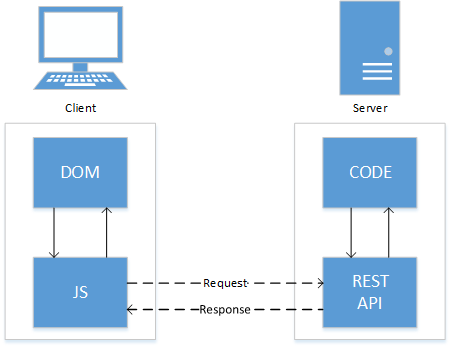
\includegraphics[width=0.6\textwidth, center]{StandDerTechnik/ClientServerJS}
    \caption[Client-Server Architektur mit Javascript]{Client-Server Architektur mit Javascript}
    \label{img:clientserverjs}
\end{figure}

In Abbildung \ref{img:clientserverjs} ist aufgezeigt, wie der Client mithilfe von Javascript mit
dem Server kommuniziert. Javascript holt
sich die Daten, die der Client benötigt und gibt diese dem DOM zum Verarbeiten weiter.

\subsection{Blazor WebAssembly}
Die Architektur von Blazor WebAssembly ist ähnlich zu den obig beschriebenen \ac{spa}s. Tatsächlich
verändert sich hierbei nur die Programmiersprache, die auf dem
Client läuft. Es handelt sich dabei um die Programmiersprache C\#, die auf dem Client
ausgeführt wird, wie im Folgenden zu sehen ist.
\begin{figure}[h]
    \centering
    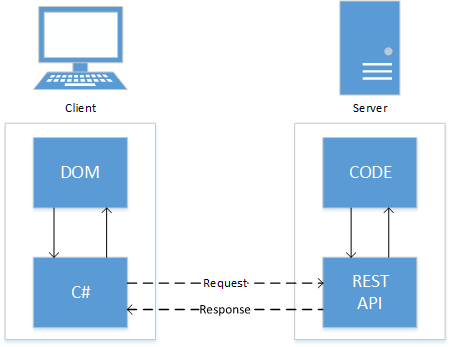
\includegraphics[width=0.6\textwidth, center]{StandDerTechnik/ClientServerCsharp}
    \caption[Blazor WebAssembly Architektur]{Blazor WebAssembly Architektur}
    \label{img:clientservercsharp}
\end{figure}
\newline
\newline
Das ganze Konzept C\# auf dem Client laufen lassen zu können, funktioniert durch
WebAssembly. WebAssembly wandelt Programmcode in nativen Bytecode um, der in einer Sandbox
im Browser ausgeführt werden kann. Dabei wird von der Sandbox aus die DOM mithilfe von
Javascript kontinuierlich manipuliert. Javascript verschwindet in dem Sinne also nicht komplett,
sondern wird lediglich ergänzt.
Da für dieses Konzept also WebAssembly vonnöten ist, kann Blazor WebAssembly nicht auf Browsern
funktionieren, die WebAssembly nicht unterstützen \cite{HierKommtBlazor}[vgl.].
\newline
\newline
Im Folgenden werden die Vor- und Nachteile von Blazor WebAssembly dargestellt:
\begin{itemize}
    \pro Sehr skalierbar
    \pro Sehr performant
    \pro Es kann komplett eigenständig auf dem Client laufen und ist nicht auf den
    Server angewiesen
    \con Große Anwendungsdatei, die auf dem Client geladen werden muss
    \con Lange Ladezeit beim ersten Aufruf
    \con Kompletter Code ist auf dem Client sichtbar
\end{itemize}

\subsection{Blazor Server}
Anders als bei Blazor WebAssembly der Fall ist, wird bei Blazor Server nicht C\# in den
Browser geladen, sondern der Code wird Serverseitig ausgeführt. Deswegen wird auch die
Web-Anwendung als SPA auf dem Server gerendert. Zum Client wird nur das JavaScript und Markup
gesendet. Die Daten und Benutzereingaben werden laufend mittels Signal R zwischen Client und Server
ausgetauscht. Dementsprechend ist es notwendig, dass immer zwischen dem Client und dem Server
eine offene Verbindung vorhanden ist \cite{HierKommtBlazor}[vgl.].
\newline
\newline
Dadurch das die komplette Seite auf dem Server gerendert wird, lädt die Seite auf dem Client sehr
schnell. Zudem muss lediglich eine kleine Javascript Datei auf den Client laden und die Seite
kann auf leistungsschwachen Clients verwendet werden.
\newline
\newline
Das ganze Konzept dieser Architektur baut drauf auf, dass beim ersten Aufruf der Seite eine
Javascript Datei names \emph{Blazor.js} auf dem Client geladen wird. Diese Datei kommuniziert
mit dem DOM und baut die Verbindung zum Server auf. Sobald die Verbindung aufgebaut ist, werden
kontinuierlich Nachrichten zwischen Client und Server ausgetauscht.

\begin{figure}[h]
    \centering
    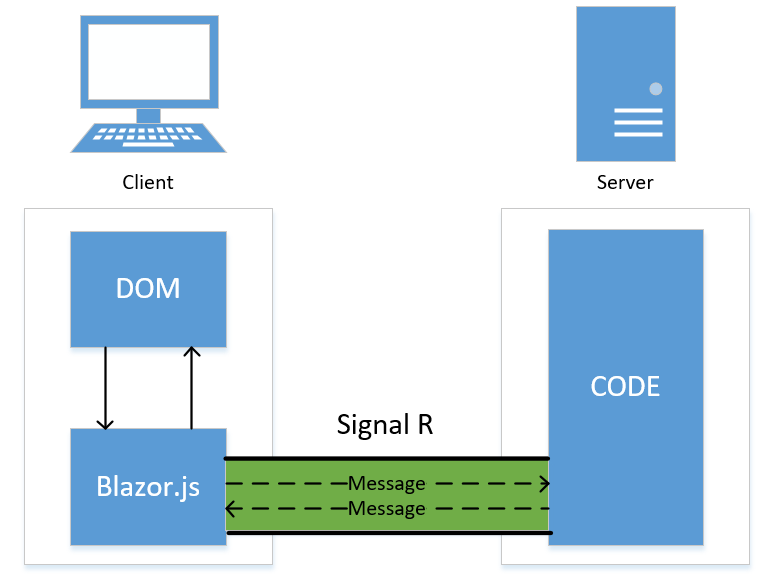
\includegraphics[width=0.6\textwidth, center]{StandDerTechnik/ClientServerSignalR}
    \caption[Serverarchitektur von Blazor]{Serverarchitektur von Blazor}
    \label{img:clientserversignalR}
\end{figure}

Im Folgenden werden die Vor- und Nachteile von Blazor Server zusammengestellt:
\begin{itemize}
    \pro Kurze Ladezeiten
    \pro Komplett browserunabhängig
    \pro Client hat keinen Zugriff auf den Sourcecode
    \pro Ist in der Lage mit leistungsschwachen Clients zu interagieren
    \con Nicht skalierbar, da alle Benutzer auf einem Server zugreifen
    \con Lange Netzwerklatenz führt zu Verzögerungen in der Benutzeroberfläche
    \con Es muss immer eine Verbindung bestehen
\end{itemize}
\section{Komponenten}
\label{subsec:komponenten}
Anders als bei Qt der Fall, basiert Blazor wie andere Web-Frameworks auf \emph{HTML} und
\emph{CSS}. Das bedeutet, dass Entwickler*innen auf jedes HTML-Element zugreifen können.
Weitergehend haben Entwickler*innen noch die Möglichkeit auf zusätzliche
Komponentenanbieter wie zum Beispiel \emph{MadBlazor} oder \emph{Ignite UI} zurückzugreifen.
\newline
\newline
Außerdem bietet Blazor zusätzlich die Möglichkeit eigene Komponenten zu erstellen. Eine
Komponente ist ein eigenständiger Teil der Benutzeroberfläche \cite{Komponenten}[vgl.].
Hinzukommend kann eine Blazor-Komponente, in zwei Varianten
vorkommen. Einmal als eine \emph{Page-Komponente} und eine \emph{Non-Page-Komponente}.
\begin{itemize}
    \item \emph{Page-Komponente} kann über die URL adressiert werden
    \item \emph{Non-Page-Komponente} kann nicht adressiert werden \cite{Komponenten}[vgl.]
\end{itemize}

\lstinputlisting[language={[Sharp]C},caption={Beispiel einer Page-Komponente},
    label=lst:counterpage]{\srcloc/Blazor/Counter.cs}

Listing \ref{lst:counterpage} zeigt eine Page-Komponete. Bei der Komponente handelt es sich um
eine Page-Komponente, da diese mit \emph{@page}
in der ersten Zeile ausgezeichnet ist.
\newline
\newline
Einer Komponente kann auch ein oder
mehrere Parameter von der Oberkomponente mitgegeben werden. Dies hat den Vorteil, dass
Komponenten mehr an Flexibilität gewinnen und somit besser wiederzuverwenden sind. Wie im
folgenden Beispiel zu sehen ist:
\lstinputlisting[language={[Sharp]C},caption={Kindkomponente},
    label=lst:childkomponente]{\srcloc/Blazor/Child.razor}

\lstinputlisting[language={[Sharp]C},caption={Elternkomponente},
    label=lst:parentkomponente]{\srcloc/Blazor/Parent.razor}

Wie in Listing \ref{lst:childkomponente} zu sehen ist, bekommt die Kindkomponente ihren Title als
Parameter übergeben. Listing
\ref{lst:parentkomponente} kann mithilfe des Title-Attributes den Title an die Kindkomponente
übergeben. Der HTML-Tag der Kindkomponente, wird durch den Dateinamen der Komponente erzeugt. Da
die Komponente \emph{Child.razor} im Projekt heißt, wird diese mittels dem
\emph{<Child>-Tag} verwendet.

\subsection{Javascript Interoperation}
\label{subsec:jsInteroperation}
Test
\section{Blazor Maui}
\label{sec:blazormaui}
Mit dem Release von .Net 6 wurde Blazor mit Maui kombiniert. Die Abkürzung \emph{Maui} steht dabei
für \emph{Multi-platform Application UI}. Mit
Blazor Maui sollen zukünftig native Desktop-  oder Mobile Applikationen mit Blazor erstellt werden
können.
\newline
\newline
Die Architektur von Blazor Maui sieht vor, dass der Blazor Code durch Maui in nativen Code
umgewandelt wird. Dieser kann dadurch auf der jeweiligen Platform ausgeführt zu werden. Was im
folgenden Bild zu erkennen ist:
\newpage
\begin{figure}[h]
    \centering
    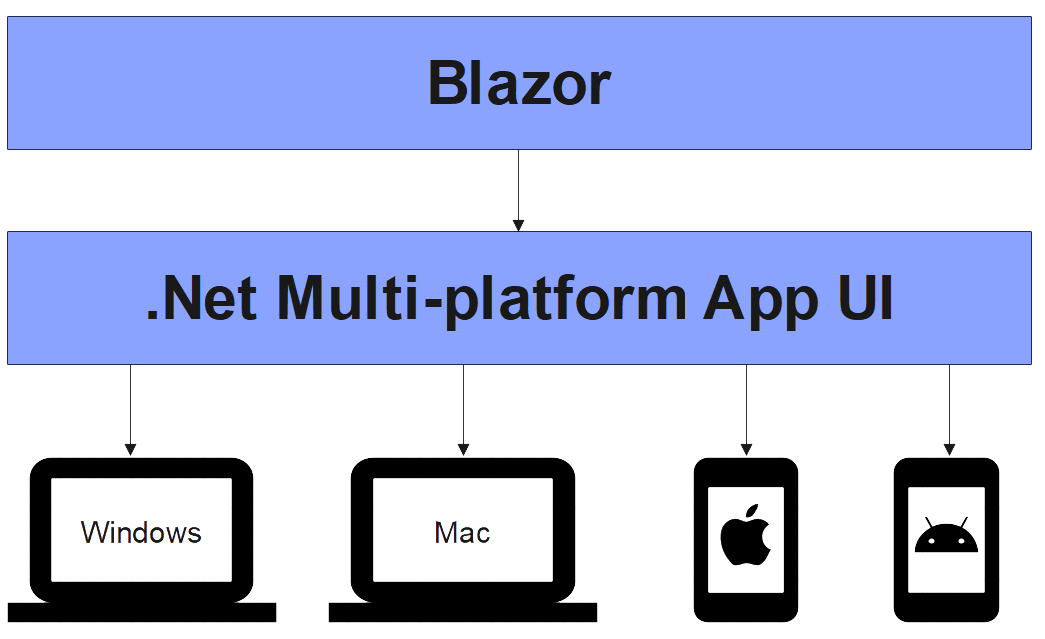
\includegraphics[width=\textwidth, center]{Blazor/BlazorMaui}
    \caption[Blazor Maui Architektur]{Blazor Maui Architektur}
    \label{img:BlazorMaui}
\end{figure}

Wie zu sehen ist, werden Windows, Mac, iOS und Android mithilfe von Maui untersützt. Linux
hingegen bleibt zu dem Zeitpunkt dieser Arbeit noch außen vor.
\newline
\newline
Aufgrund dessen, das Linux zum derweiligen Zeitpunkt noch nicht unterstützt wird, und Non-Deeply
Embedded System meist auf Linux basieren, wird Blazor Maui nicht weitergehend in dieser Arbeit
behandelt.
\chapter{Raspberry Pi mit .Net Core und Blazor}
\label{chp:RaspMitBlazor}
In diesem Kapitel soll nun ein einfaches Open Embedded System mithilfe von Blazor auf einem
Raspberry Pi 4B erstellt werden. Dabei soll gezeigt werden, welche Entwicklungsumgebung, unter
anderem, genutzt werden kann und was auf dem Target installiert werden muss.

%sections
\section{Entwicklungsumgebung}
\label{sec:entwicklungsumgebung}
Test
\section{Installation}
\label{sec:installation}
Test

%\section{Programmieren mit .Net Core}
\label{sec:progmitnet}
Test

\section{Blazor Demo Anwendung}
\label{sec:blazordemo}
Nachdem in der letzten Sektion \emph{\nameref{sec:installation}} .Net installiert wurde, soll in
dieser Sektion eine beispielhafte Blazor Anwendung auf dem Raspberry Pi erstellt werden. Die
Anwendung wird auf der \emph{Blazor Server} Architektur basieren. Dabei sollen kontinuierlich
Daten von dem Raspberry Pi abgefragt und auf der Benutzeroberfläche repräsentiert werden.
\subsection{Erstellen des Projektes}
\label{subsec:erstellenProject}
Um eine Blazor Anwendung zu erstellen, gibt es zwei Möglichkeiten. Zum einem vom \emph{Scratch}
aus, aus einer einfachen Konsolen Anwendung, um den notwendigen Code zu implementiert, oder zum
anderen mit hilfe eines Templates. Microsoft bietet einige Templates für verschiedenste
Anwendungen an, die alle samt mit der Installation von .Net kommen.
\newline
\newline
Um nun die Anwendung mithilfe des Templates zu erstellen, muss der folgende Befehl in dem Teminal
eingegeben werden:

\begin{zitat}
    dotnet new blazorserver -o MyApp --no-https
\end{zitat}

Dieser Befehl erstellt eine neue Blazor Server Anwendung, mit dem Namen \emph{MyApp} und
konfiguriert die Anwendung ohne das Https Protokol. Der name sowie, dass kein Https konfiguriert
wird, sind optionale Parameter, die nicht mit angegeben werden müssen. Nachdem die Anwendung 
erfolgreich Installiert wurde, muss noch die Codezeile \emph{webBuilder.UseUrls("Http://*:5000");
} in der \emph{Program.cs} angegeben werden, um die Anwendung für alle Geräte im LAN verfügbar
ist. Der Code in der \emph{Program.cs} sieht dann folgendermaßen aus:

\begin{lstlisting}[language={[Sharp]C}, caption=Program.cs Code,
    label=lst:programCsCode]
    public class Program
    {
        // Main

        public static IHostBuilder CreateHostBuilder(string[] args) =>
            Host.CreateDefaultBuilder(args)
                .ConfigureWebHostDefaults(webBuilder =>
                {
                    webBuilder.UseStartup<Startup>();
                    webBuilder.UseUrls("Http://*:5000"); // <----
                });
    }
\end{lstlisting}

Mit dem Befehl \emph{dotnet run} kann die Anwendung dann gestartet werden. Sobald das Programm
gestartet ist, kann mit dem Link \emph{http://<ip>:5000} die Seite erreicht werden. Sollte alles
geklappt haben sollte nun die Seite, mit den schon vom Template gegebenen Komponenten, wie folgt
angezeigt werden:

\begin{figure}[h]
    \centering
    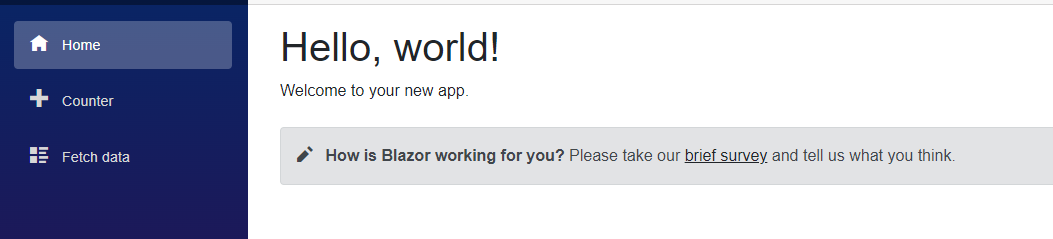
\includegraphics[width=\textwidth, center]{BlazorRasp/ServerTemplate}
    \caption[Blazor Server Template]{Blazor Server Template}
    \label{img:BlazorServerTemplate}
\end{figure}
\subsection{Microsoft IoT}
\label{subsec:MicrosoftIot}
Damit mit dem Raspberry Pi kommuniziert werden kann, können Bibliotheken verwendet werden.
Microsoft bietet eine IoT Bibliothek an, mit der die Sensoren oder die LEDs auf
dem Gerät angesteuert werden können. Die Bibliothek kann wie folgt in das Projekt eingebunden
werden:

\begin{lstlisting}[language={[Sharp]C}, caption=IoT NuGet Package,
    label=lst:IotNugetPackage]
    <ItemGroup>
    <PackageReference Include="Iot.Device.Bindings" Version="1.5.0-*" />
  </ItemGroup>
\end{lstlisting}

Das folgende beispielhafte Konsolenprogramm demonstriert, wie auf die Daten zugegriffen werden kann:

\begin{lstlisting}[language={[Sharp]C}, caption=SenseHat Beispielprogramm,
    label=lst:SenseHatBeispielProgramm]
    public class Program
    {
        static void Main(string[] args)
        {
            using SenseHat _senseHat = new();

            Console.WriteLine($"Temperatur: {_senseHat.Temperature.DegreesCelsius:0.#}\u00B0C");
            Console.WriteLine($"Temperatur 2: {_senseHat.Temperature2.DegreesCelsius:0.#}\u00B0C");
            Console.WriteLine($"Luftdruck: {_senseHat.Pressure.Hectopascals:0.##} hPa");
            Console.WriteLine($"Luftfeuchtigkeit: {_senseHat.Humidity.Percent:0.#}%");
        }
    }
\end{lstlisting}

Der Output durch obiges Programm sieht wie folgt aus:

\begin{zitat}
    Temperatur: 38,4°C
    \newline
    Temperatur 2: 38,5°C
    \newline
    Luftdruck: 984,03 hPa
    \newline
    Luftfeuchtigkeit: 31\%
\end{zitat}
\subsection{Raspberry Pi Daten Anzeigen}
\label{subsec:DatenAnzeigen}
In dieser Sektion soll nun die Logik implementiert werden, um die Daten, die vom Raspberry Pi
kommen, auf der Benutzeroberfläche anzuzeigen. Dafür wird ein \emph{Timer} implementiert werden, der
jede Sekunde auslöst, um dann die Daten zu lesen.
\newline
\newline
Damit etwas auf der Benutzeroberfläche angezeigt werden kann, muss das \emph{Html-Markup}
implementiert werden:

\begin{lstlisting}[language={[Sharp]C}, caption=Html-Markup,
    label=lst:HtmlMarkup]
<div class="divHeader">
    <div>
        <h1>Raspberry Pi</h1>

        <h2>Uhrzeit: @_uhrzeit</h2>
    </div>

    <div>
        <h3>Temperature Sensor 1: @_temperatur</h3>
        <h3>Temperature Sensor 2: @_temperatur2</h3>
        <h3>Luftdruck: @_pressure</h3>
        <h3>Luftfeuchtigkeit: @_humidity</h3>
    </div>
</div>
\end{lstlisting}

Dabei signalisiert das \emph{@<name>}, dass es sich dabei um eine Variable handelt, die im Code
deklariert wurde.
\newline
\newline
Weitergehend bietet Blazor verschiedene \emph{Render-Funktionen} die nach bestimmten ereignissen
aufgerufen werden. Wie zum Beispiel die \emph{OnInitializedAsync}, die aufgerufen wird, wenn die
Komponente geladen wird. Diese \emph{OnInitializedAsync} kann nun dazu gebraucht werden, um die
Variablen zu initialisieren.

\begin{lstlisting}[language={[Sharp]C}, caption=Render-Funktion: OnInitializedAsync,
    label=lst:OnInitializedAsync]
    protected override Task OnInitializedAsync()
    {
        _senseHat = new();
        _cultureInfo = new("de-DE");
        _uhrzeit = DateTime.Now.ToString("HH:mm:ss", _cultureInfo);

        _temperatur = string.Empty;
        _temperatur2 = string.Empty;
        _pressure = string.Empty;
        _humidity = string.Empty;

        return base.OnInitializedAsync();
    }
\end{lstlisting}

Nun soll zudem noch eine Hilfsfunktion \emph{SetRaspValues} geschaffen werden, die die Daten
ausliest. Diese Funktion wird dann auch in der \emph{OnInitializedAsync} Funktion aufgerufen.

\begin{lstlisting}[language={[Sharp]C}, caption=Funktion: SetRaspValues,
    label=lst:SetRaspValues]
    private void SetRaspValues()
    {
        _temperatur = $"{_senseHat.Temperature.DegreesCelsius:0.#}\u00B0C";
        _temperatur2 = $"{_senseHat.Temperature2.DegreesCelsius:0.#}\u00B0C";
        _pressure = $"{_senseHat.Pressure.Hectopascals:0.##} hPa";
        _humidity = $"{_senseHat.Humidity.Percent:0.#}%";
    }
\end{lstlisting}

Damit die Daten jedoch nicht nur einmal am Anfang gelesen werden, sondern sich kontinuierlich
aktuallisieren, soll ein \emph{Timer} jede Sekunde getriggert werden, um die Daten neu zu lesen
und dem \emph{DOM} mitzuteilen, dass sich der \emph{State} der Seite geändert hat.

\begin{lstlisting}[language={[Sharp]C}, caption=Timer: ReadTimer,
    label=lst:ReadTimer]
    private void StartTimer()
    {
        _readTimer = new(1000);
        _readTimer.Elapsed += GetData;
        _readTimer.Enabled = true;
    }

    private void GetData(Object source, System.Timers.ElapsedEventArgs e)
    {
        _uhrzeit = DateTime.Now.ToString("HH:mm:ss", cultureInfo);
        SetRaspValues();
        InvokeAsync(StateHasChanged);
    }
\end{lstlisting}

Wichtig hierbei ist jedoch, dass die Funktion \emph{StateHasChanged} manuell aufgerufen
wurde. Dies übernimmt Blazor normalerweise schon automatisch, wenn sich Variablen der Komponente
verändern, die angezeigt werden aber da hier die Variablen nicht auf dem \emph{Ui-Thread} geändert
wurden, muss manuell angegeben werden, dass sich der \emph{State} geändert hat.
\newline
\newline
Der momentane Stand der Seite zieht so aus:

\begin{figure}[h]
    \centering
    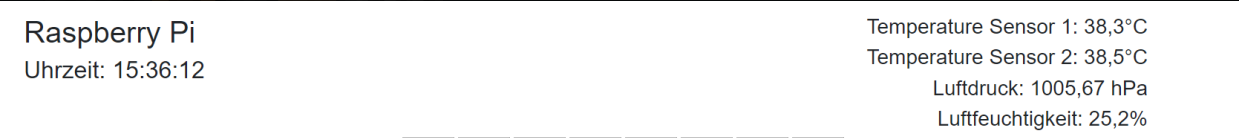
\includegraphics[width=\textwidth, center]{BlazorRasp/BlazorDatenAnzeigen}
    \caption[Zwischenstand der Blazor Demo]{Zwischenstand der Blazor Demo}
    \label{img:BlazorDatenAnzeigen}
\end{figure}
\subsection{LED-Matrix ansteuern}
\label{subsec:ledMatrix}
In dieser Sektion soll eine \emph{8x8 Button-Matrix} erstellt werden, die die \emph{8x8
LED-Matrix} auf dem Sensehat des Raspberry Pi repräsentieren soll. Dabei soll der vorhandene
Joystick auf dem Sensehat genutzt werden, um über die Button-Matrix zu navigieren und die
LEDs zu platzieren.
\newline
\newline
Da Blazor die \emph{Razor-Syntax} verwendet, kann jegliche C\# Kontrollstruktur im
\emph{HTML-Markup} verwendet werden. So kann dies wie folgt genutzt werden, um die \emph{8x8
Button-Matrix} zu erzeugen:

\begin{lstlisting}[language={[Sharp]C}, caption=Button-Matrix,
    label=lst:ButtonMatrix]
<div class="divGrid">
    @for (var y = 0; y < LengthY; y++)
    {
        @for (var x = 0; x < LengthX; x++)
        {
            int copyY = y;
            int copyX = x;
            <Button class="buttonBox @classes[copyY,copyX]"/>
        }
    }
</div>
\end{lstlisting}

Das \emph{@classes} Element ist ein Zwei-Dimensionales Array aus Strings, mit der
CSS-Klassen hinzugefügt und wieder gelöscht werden sollen. Um zu ermitteln, welcher
Joystick-Button betätigt wurde, soll ein weiterer
\emph{Timer} zum Einsatz kommen. Dieser Timer soll alle 15 Millisekunden ausgelöst werden.

\begin{lstlisting}[language={[Sharp]C}, caption=Timer: _setButtonTimer,
    label=lst:ButtonTimer]
    private void StartTimer()
    {
        // More Code

        _setButtonTimer = new(15);
        _setButtonTimer.Elapsed += WriteStateToChannel;
        _setButtonTimer.Enabled = true;
    }


    private async void WriteStateToChannel(Object source, System.Timers.ElapsedEventArgs e)
    {
        if((ticks - lastTicks) > 9){
            _senseHat.ReadJoystickState();
            if(_senseHat.HoldingButton){
                await _stateChannel.Writer.WriteAsync(JoystickState.Holding);
            }
            else if(_senseHat.HoldingUp){
                await _stateChannel.Writer.WriteAsync(JoystickState.Up);
            }
            else if(_senseHat.HoldingDown){
                await _stateChannel.Writer.WriteAsync(JoystickState.Down);
            }
            else if(_senseHat.HoldingLeft){
                await _stateChannel.Writer.WriteAsync(JoystickState.Left);
            }
            else if(_senseHat.HoldingRight){
                await _stateChannel.Writer.WriteAsync(JoystickState.Right);
            }
            lastTicks = ticks;
        }
        ticks++;
    }
\end{lstlisting}

Bei \emph{JoystickState} handelt es sich um ein Enum, welches den \emph{State} des Joysticks
repräsentieren soll. Wie zu sehen ist, wird der aktuelle \emph{State} des Joysticks gelesen, um
das Ergebnis in einen \emph{Channel} zu schreiben.
\newline
\newline
Für die Verarbeitung des \emph{States}, wird in \emph{OnInitializedAsync} ein Task gestartet, der
in einer Endlosschleife läuft und darauf warte bis etwas in den \emph{Channel} hinzugefügt
wird. Sobald sich der \emph{State} geändert hat, wird entweder die Position berechnet oder
die LED an dieser Position leuchtet in einer neuen Farbe.

\begin{lstlisting}[language={[Sharp]C}, caption=Task zum Verarbeiten des States,
    label=lst:StateTask]
        _setButtonTask = Task.Run(async () =>
        {
            while (true)
            {
                if(cancellationToken.IsCancellationRequested)
                    cancellationToken.ThrowIfCancellationRequested();
                var state = await _stateChannel.Reader.ReadAsync();
                int x = 0;
                int y = 0;
                if(state == JoystickState.Holding){
                    SetButtonBackground(_currentX, _currentY);
                }
                else if(state == JoystickState.Up){
                    y--;
                }
                else if(state == JoystickState.Down){
                    y++;
                }
                else if(state == JoystickState.Left){
                    x--;
                }else if(state == JoystickState.Right){
                    x++;
                }
                SetPositions(x, y);
                RemoveButtonBorder(_previousX, _previousY);
                SetButtonBorder(_currentX, _currentY);
                await InvokeAsync(StateHasChanged);
            }
        });

    private void SetButtonBackground(int x, int y)
    {
        if (classes[y, x].Contains(" setBackground"))
        {
            _senseHat.SetPixel(x, y, Color.Blue);
            classes[y, x] = classes[y, x].Replace(" setBackground", string.Empty);
        }
        else
        {
            _senseHat.SetPixel(x, y, Color.Red);
            classes[y, x] += " setBackground";
        }
    }
\end{lstlisting}

Wie zu erkennen ist, wird die LED und der Button je
nach vorherigem Zustand entweder Blau oder Rot. Die entstandene Anwendung sieht dann wie folgt aus:

\begin{figure}[h]
    \centering
    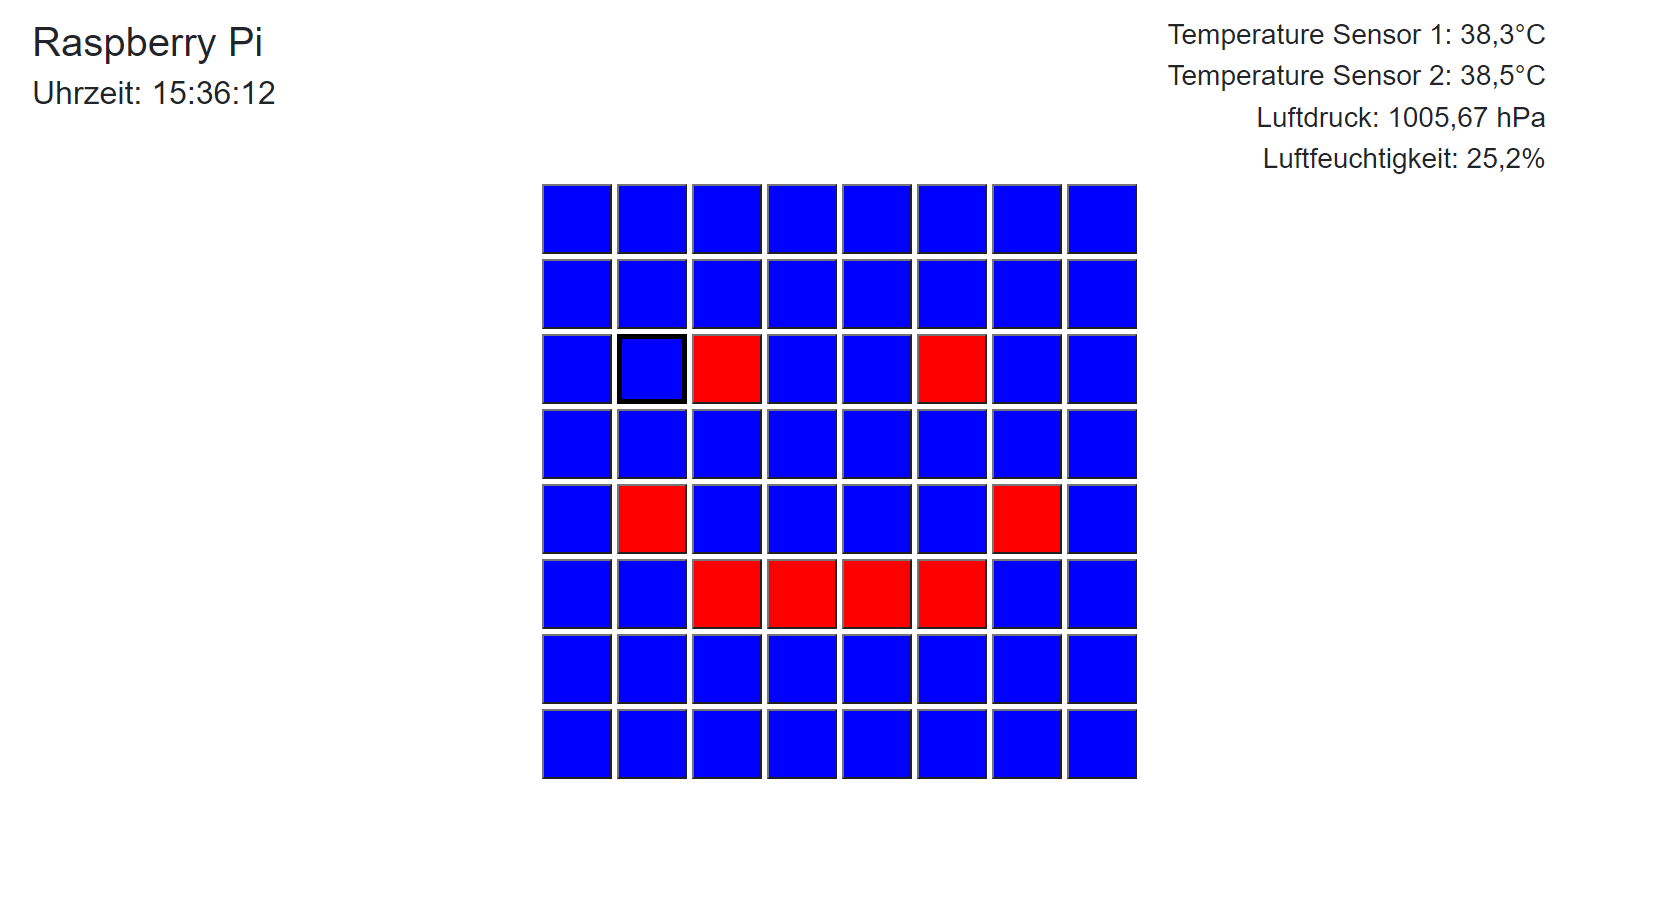
\includegraphics[width=\textwidth, center]{BlazorRasp/Demo}
    \caption[Blazor Demo]{Blazor Demo}
    \label{img:BlazorDatenAnzeigen}
\end{figure}

Da nur technisch relevante Code Abschnitte in diesem Kapitel präsentiert wurden, ist der
komplette Code im Anhang \ref{lst:DemoCode} zu finden.
\chapter{Analyse}
\label{chp:analyse}
Test
\chapter{Fazit}
\label{chp:fazit}
Test
\chapter{Ausblick}
\label{chp:ausblick}
Abschließend soll noch ein kurzer Ausblick über die weitere Entwicklung von Benutzeroberflächen für
Non-Deeply Embedded Systems gegeben werden. Die beiden vorgestellten Frameworks dieser Arbeit
eignen sich beide für die Entwicklung einer Benutzeroberfläche. Jedoch muss hier differenziert
werden, welche Kriterien die Benutzeroberfläche erfüllen muss.

In dem Fall, dass die Performance sehr wichtig ist, sollte auf das Framework Qt in
Kombination mit C++ zurückgegriffen werden. Sollte jedoch ein schneller Entwicklungsprozess
vonnöten sein, ist das Framework Blazor definitiv eine gute Alternative.

In dieser Arbeit wurde zudem noch die Blazor Maui-Architektur vorgestellt, die aufgrund der nicht
vorhandenen Kompatibilität mit Linux, nicht weiter betrachtet werden konnte. Hier bleibt es
abzuwarten, ob Microsoft Linux mit \emph{Blazor} unterstützten wird. Sollte Linux in Zukunft
von Blazor Maui profitieren, so sollte eine solche Analyse erneut durchgeführt werden.
%\listoftodos

\chapter{Kapitel 1}
\label{chap:kapitel1}
Lorem ipsum dolor sit amet, consetetur sadipscing elitr, sed diam nonumy eirmod tempor invidunt ut labore et dolore magna aliquyam erat, sed diam voluptua. At vero eos et accusam et justo duo dolores et ea rebum. Stet clita kasd gubergren, no sea takimata sanctus est Lorem ipsum dolor sit amet. Lorem ipsum dolor sit amet, consetetur sadipscing elitr, sed diam nonumy eirmod tempor invidunt ut labore et dolore magna aliquyam erat, sed diam voluptua. At vero eos et accusam et justo duo dolores et ea rebum. Stet clita kasd gubergren, no sea takimata sanctus est Lorem ipsum dolor sit amet \cite{Fowler2014}.

	\section{Microservices}
	\label{sec:microservices}
	Lorem ipsum dolor sit amet, consetetur sadipscing elitr, sed diam nonumy eirmod tempor invidunt ut labore et dolore magna aliquyam erat, sed diam voluptua. At vero eos et accusam et justo duo dolores et ea rebum. Stet clita kasd gubergren, no sea takimata sanctus est Lorem ipsum dolor sit amet. Lorem ipsum dolor sit amet, consetetur sadipscing elitr, sed diam nonumy eirmod tempor invidunt ut labore et dolore magna aliquyam erat, sed diam voluptua. At vero eos et accusam et justo duo dolores et ea rebum. Stet clita kasd gubergren, no sea takimata sanctus est Lorem ipsum dolor sit amet. Referenz zur Abbildung \ref{img:microprofile}.
	\begin{figure}[h]
		\centering
		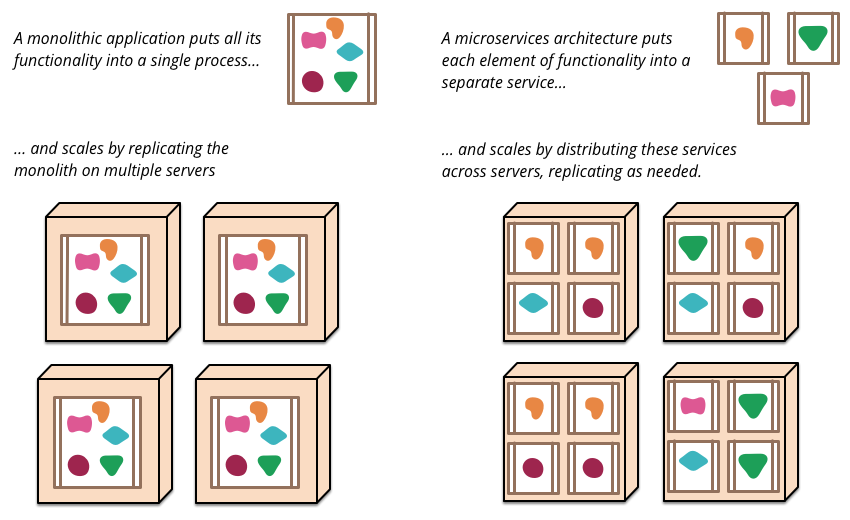
\includegraphics[width=\textwidth, center]{kapitel1/monolith_vs_microservices}
		\caption[Beschreibung für Verzeichnis]{Bildunterschrift}
		\label{img:microprofile}
	\end{figure}
	
	\subsection{Was sind Microservices}
	Lorem ipsum dolor sit amet, consetetur sadipscing elitr, sed diam nonumy eirmod tempor invidunt ut labore et dolore magna aliquyam erat, sed diam voluptua. At vero eos et accusam et justo duo dolores et ea rebum. Stet clita kasd gubergren, no sea takimata sanctus est Lorem ipsum dolor sit amet. Lorem ipsum dolor sit amet, consetetur sadipscing elitr, sed diam nonumy eirmod tempor invidunt ut labore et dolore magna aliquyam erat, sed diam voluptua. At vero eos et accusam et justo duo dolores et ea rebum. Stet clita kasd gubergren, no sea takimata sanctus est Lorem ipsum dolor sit amet \cite{Reese2009}.
	
	\paragraph{Klein und spezialisiert} Lorem ipsum dolor sit amet, consetetur sadipscing elitr, sed diam nonumy eirmod tempor invidunt ut labore et dolore magna aliquyam erat, sed diam voluptua. At vero eos et accusam et justo duo dolores et ea rebum. Stet clita kasd gubergren, no sea takimata sanctus est Lorem ipsum dolor sit amet. Lorem ipsum dolor sit amet, consetetur sadipscing elitr, sed diam nonumy eirmod tempor invidunt ut labore et dolore magna aliquyam erat, sed diam voluptua. At vero eos et accusam et justo duo dolores et ea rebum. Stet clita kasd gubergren, no sea takimata sanctus est Lorem ipsum dolor sit amet.
	
	\paragraph{Eigenständig} Lorem ipsum dolor sit amet, consetetur sadipscing elitr, sed diam nonumy eirmod tempor invidunt ut labore et dolore magna aliquyam erat, sed diam voluptua. At vero eos et accusam et justo duo dolores et ea rebum. Stet clita kasd gubergren, no sea takimata sanctus est Lorem ipsum dolor sit amet. Lorem ipsum dolor sit amet, consetetur sadipscing elitr, sed diam nonumy eirmod tempor invidunt ut labore et dolore magna aliquyam erat, sed diam voluptua. At vero eos et accusam et justo duo dolores et ea rebum. Stet clita kasd gubergren, no sea takimata sanctus est Lorem ipsum dolor sit amet. Verweis auf Anhang \ref{appendix:anhanga} \nameref{appendix:anhanga}
 % Externe Datei einbinden
%\chapter{Kapitel 2}
\label{chap:kapitel2}
Eine Abkürzung \ac{cd}, \ac{ci}. Ausgeschrieben \acl{cd}. Verweis zu einem File-Listing \ref{lst:crypter} oder einem Listing im Textfluss \ref{lst:Rggplot} und ein Inline-Listing \lstinline|print("Hello World")|.

\lstinputlisting[language=Java,caption={Ein Listing},label=lst:crypter]{\srcloc/Crypter.java}

\begin{lstlisting}[language=R,caption=Beispielaufruf ldply-Funktion in R, label=lst:Rggplot]
ggplot(data = data, mapping = aes(x=timestamp, y=score) + geom_line()
\end{lstlisting}
			 % Externe Datei einbinden
% ------------------------------------------------------------------

\label{lastpage}

% Neue Seite
\cleardoublepage

% Backmatter mit normalem Zeilenabstand setzen
\singlespacing

% Römische Ziffern für die "Back-Matter", fortlaufend mit "Front-Matter"
\pagenumbering{roman}
%\setcounter{page}{\value{frontmatterpage}}
\setcounter{page}{0}
% Abkürzungsverzeichnis
\addchap{\hsmaabbreviations}
\begin{acronym}[IEEE]
	\acro{cd}[CD]{Continuous Delivery}
	\acro{ci}[CI]{Continuous Integration}
	\acro{gui}[GUI]{Graphical User Interface}
	\acro{moc}[moc]{meta object compiler}
	\acro{spa}[SPA]{Single Page Application}
\end{acronym}


% Tabellenverzeichnis erzeugen
\cleardoublepage
\phantomsection
\addcontentsline{toc}{chapter}{\hsmalistoftables}
\listoftables

% Abbildungsverzeichnis erzeugen
\cleardoublepage
\phantomsection
\addcontentsline{toc}{chapter}{\hsmalistoffigures}
\listoffigures

% Listingverzeichnis erzeugen
\cleardoublepage
\phantomsection
\addcontentsline{toc}{chapter}{\hsmalistings}
\lstlistoflistings

% Literaturverzeichnis erzeugen
\begin{flushleft}
\printbibliography[heading=bibintoc, title={Literatur}]
\end{flushleft}

% Index ausgeben. Wenn Sie keinen Index haben, entfernen Sie einfach
% diesen Teil.
%\cleardoublepage
%\phantomsection
%\addcontentsline{toc}{chapter}{\hsmaindex}
%\printindex

% Anhang. Wenn Sie keinen Anhang haben, entfernen Sie einfach
% diesen Teil.
\appendix
\chapter{Ein Anhang}
\label{appendix:anhanga}

Referenz zu Tabelle \ref{table:topbeatmetricssystem}.

\begin{table}[ht]
	\centering
	\begin{tabularx}{\textwidth}{msb}
		\textbf{Bezeichnung} 	& \textbf{Typ} 		& \textbf{Beschreibung} 	\\ \hline 
		load.load1 				& float	  			& The load average over 1 minute.				\\ \rowcolor{Gray}
		load.load5 				& float 			& The load average over 5 minutes.				\\ 
		load.load15				& float 			& The load average over 15 minutes.				\\ \rowcolor{Gray}
		cpu.user				& int	 			& The amount of CPU time spent in user space.  	\\ 
		cpu.user\_p				& float	 			& The percentage of CPU time spent in user space. On multi-core systems, you can have percentages that are greater than 100\%. For example, if 3 cores are at 60\% use, then the cpu.user\_p will be 180\%.	\\ \rowcolor{Gray}
		cpu.system				& int	 			& The amount of CPU time spent in kernel space.	\\ 
		cpu.system\_p			& float	 			& The percentage of CPU time spent in kernel space.	\\ \rowcolor{Gray}
		mem.total				& int	 			& Total memory.								  	\\ 
		mem.used				& int	 			& Used memory.								  	\\ \rowcolor{Gray}
		mem.free				& int	 			& Available memory.							  	\\ 
		mem.used\_p				& float	 			& The percentage of used memory.			
	\end{tabularx}
	\caption{Tabellenunterschrift}
	\label{table:topbeatmetricssystem}
\end{table}

\begin{figure}[h]
	\centering
	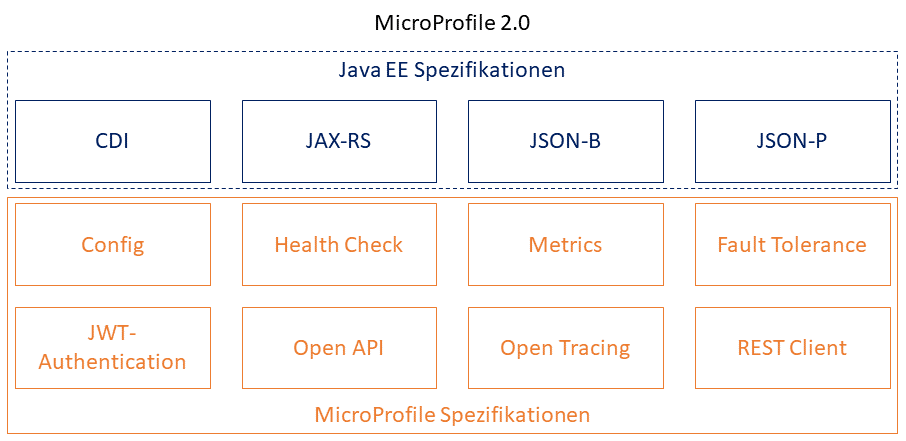
\includegraphics[width=\textwidth, center]{anhanga/microprofile_components}
	\caption[Beschreibung für Verzeichnis2]{Bildunterschrift2}
	\label{img:microprofile_components}
\end{figure}

\end{document}
